%; whizzy section -pdf xpdf -latex ./whizzypdfptex.sh
% latex beamer presentation.
% platex, latex-beamer でコンパイルすることを想定。

%     Tokyo Debian Meeting resources
%     Copyright (C) 2007 Junichi Uekawa
%                   2007 Nobuhiro Iwamatsu
%                   2007 Aya Komuro

%     This program is free software; you can redistribute it and/or modify
%     it under the terms of the GNU General Public License as published by
%     the Free Software Foundation; either version 2 of the License, or
%     (at your option) any later version.

%     This program is distributed in the hope that it will be useful,
%     but WITHOUT ANY WARRANTY; without even the implied warranty of
%     MERCHANTABILITY or FITNESS FOR A PARTICULAR PURPOSE.  See the
%     GNU General Public License for more details.

%     You should have received a copy of the GNU General Public License
%     along with this program; if not, write to the Free Software
%     Foundation, Inc., 51 Franklin St, Fifth Floor, Boston, MA  02110-1301 USA

% 実行順番
% sudo  ~/bin/usb-macbook-ir.c &
% real presentation (shell-command (concat "DISPLAY=:0.1 xpdf -fullscreen " (replace-regexp-in-string "tex$" "pdf"(buffer-file-name)) "&"))
% DISPLAY=:0.1 xpdf -fullscreen

\documentclass[cjk,dvipdfmx,12pt]{beamer}
\usetheme{Tokyo}
\usepackage{ulem}
\usepackage{tabularx}

\usepackage{fancybox}
\usepackage{fancyvrb}
\usepackage{float}
\usepackage[english]{babel}

% commandline環境を定義。画面入出力についてはcommandline環境
% で表記する
\newenvironment{commandline}%
{\VerbatimEnvironment
  \begin{Sbox}\begin{minipage}{0.9\hsize}\begin{fontsize}{7.3}{7.3} \begin{BVerbatim}}%
{\end{BVerbatim}\end{fontsize}\end{minipage}\end{Sbox}
  \setlength{\fboxsep}{8pt}
% start on a new paragraph

\vspace{6pt}% skip before
\fcolorbox{dancerdarkblue}{dancerlightblue}{\TheSbox}

\vspace{6pt}% skip after
}
%end of commandline

\definecolor{dancerdarkblue}{rgb}{0,0.08,0.45}
\definecolor{dancernormalblue}{rgb}{0.8,0.9,0.95}
\definecolor{dancerlightblue}{rgb}{0.8,0.95,1}


%  preview (shell-command (concat "evince " (replace-regexp-in-string "tex$" "pdf"(buffer-file-name)) "&"))
%  presentation (shell-command (concat "xpdf -fullscreen " (replace-regexp-in-string "tex$" "pdf"(buffer-file-name)) "&"))

%http://www.naney.org/diki/dk/hyperref.html
%日本語EUC系環境の時
\AtBeginDvi{\special{pdf:tounicode EUC-UCS2}}
%シフトJIS系環境の時
%\AtBeginDvi{\special{pdf:tounicode 90ms-RKSJ-UCS2}}

\title{東京エリア Debian 勉強会}
\subtitle{資料}
\author{岩松 信洋 iwamatsu@debian.or.jp\\IRC nick: iwamatsu}
\date{2007年9月15日}
\logo{
\includegraphics[width=8cm]{image200607/openlogo-light.eps}}


% 間のタイトルページ用
\newcommand{\emtext}[1]{
\begin{frame}{}

\begin{minipage}{0.55\hsize}
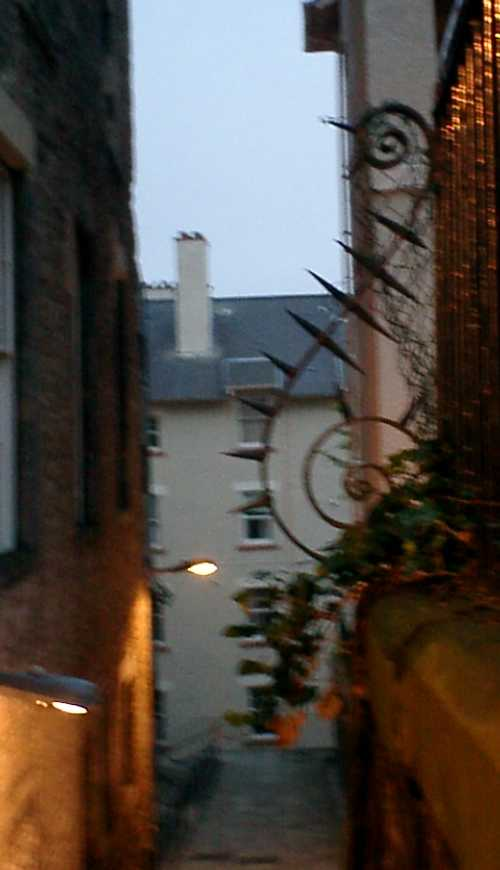
\includegraphics[width=1\hsize]{image200707/gurutitle.jpg}
\end{minipage}
\begin{minipage}{0.39\hsize}
 {\Huge #1
 }
\end{minipage}
\end{frame}
}

% 三択問題用
\newcounter{santakucounter}
\newcommand{\santaku}[5]{%
\addtocounter{santakucounter}{1}
\frame{\frametitle{問題\arabic{santakucounter}. #1}
%問題\arabic{santakucounter}. #1
\begin{minipage}[t]{0.8\hsize}
 \begin{itemize}
 \item
      \begin{minipage}{0.2\hsize}
      
\includegraphics[width=0.9\hsize]{image200703/janken-A.png}\end{minipage}
       \begin{minipage}{0.6\hsize}
       A #2\end{minipage}\\
 \item
      \begin{minipage}{0.2\hsize}
      
\includegraphics[width=0.9\hsize]{image200703/janken-B.png}\end{minipage}
       \begin{minipage}{0.6\hsize}
       B #3\end{minipage}\\
 \item
      \begin{minipage}{0.2\hsize}
      
\includegraphics[width=0.9\hsize]{image200703/janken-C.png}\end{minipage}
       \begin{minipage}{0.6\hsize}
       C #4\end{minipage}\\
 \end{itemize}
\end{minipage}
}
\frame{\frametitle{問題\arabic{santakucounter}. #1}
%問題\arabic{santakucounter}. #1
\begin{minipage}[t]{0.8\hsize}
\begin{itemize}
 \item
      \begin{minipage}{0.2\hsize}
      
\includegraphics[width=0.9\hsize]{image200703/janken-A.png}\end{minipage}
       \begin{minipage}{0.6\hsize}
       A #2\end{minipage}\\
 \item
      \begin{minipage}{0.2\hsize}
      
\includegraphics[width=0.9\hsize]{image200703/janken-B.png}\end{minipage}
       \begin{minipage}{0.6\hsize}
       B #3\end{minipage}\\
 \item
      \begin{minipage}{0.2\hsize}
      
\includegraphics[width=0.9\hsize]{image200703/janken-C.png}\end{minipage}
       \begin{minipage}{0.6\hsize}
       C #4\end{minipage}\\
\end{itemize}
\end{minipage}
\begin{minipage}[t]{0.15\hsize}
答えは:

\vspace{1cm}

  {\huge \hspace{1cm}#5}
  \hspace{-6cm}\includegraphics[width=4cm]{image200703/janken-#5.png}
 \end{minipage}}
}

\begin{document}
\frame{\titlepage{}}

\section{Intro}

\begin{frame}
 \frametitle{Agenda}
\begin{minipage}[t]{0.45\hsize}
  \begin{itemize}
  \item 注意事項
	\begin{itemize}
	 \item 飲食禁止
	 \item 政治/宗教/営利活動禁止
	\end{itemize}
  \item quiz
  \item 最近のDebian関連のイベント
	\begin{itemize}
	 \item 前回
	 \item コミケ
	 \item 1st Debian JP BSP
	\end{itemize}
 \end{itemize}
\end{minipage}
\begin{minipage}[t]{0.45\hsize}
 \begin{itemize}
  \item Exim
  \item MTA/MUA,ネットワークプロトコル
 \end{itemize}
\end{minipage}
\end{frame}

\section{最近}

\begin{frame}
 \frametitle{前回のAgenda}
\begin{minipage}[t]{0.45\hsize}
  \begin{itemize}
  \item 注意事項
	\begin{itemize}
	 \item 飲食禁止
	 \item 政治/宗教/営利活動禁止
	\end{itemize}
  \item quiz
  \item 最近のDebian関連のイベント
	\begin{itemize}
	 \item 前回
	 \item OSC-Kansai
	\end{itemize}
 \end{itemize}
\end{minipage}
\begin{minipage}[t]{0.45\hsize}
 \begin{itemize}
  \item cdn.debian.or.jp
  \item 最近はまったこと
 \end{itemize}
\end{minipage}
\end{frame}

\section{DWN quiz}
\begin{frame}{Debian 常識クイズ}

Debian の常識、もちろん知ってますよね?
しらないとはずかしいけどしらないとは言えないいろいろなこと、
会長がこの目で確認しちゃうぞ!


今回の出題範囲は\url{debian-devel@lists.debian.org} に投稿された内容からです。
\end{frame}

\subsection{問題}

\santaku
{Albert Einstein が作った Debian ベースのディストリビューションは何か}
{ice linux}
{fantasy linux}
{fire linux}
{A}

\santaku
{そしてこのAlbert Einstein が debian-devel で質問した内容は何でしょう}
{なぜ Internet Explorer が Debian にないのですか。}
{なぜ Opera が Debian にないのですか。}
{なぜ Safari が Debian にないのですか。}
{B}

\santaku
{Luk Claes が RCバグについて提案したのはどのような内容か}
{RCバグが出たパッケージのメンテナへのペナルティを考える提案}
{RCバグの 0-day NMU についての提案}
{RCバグをいかにして無視するか、という HowTo.}
{B}

\santaku
{packages.debian.orgにいろいろ新機能が追加されました。どのような機能が追加されましたか}
{メールフォワード機能}
{カルマ付加機能}
{Webからパッケージ乗っ取り機能}
{A}

\section{最近の話題}

\emtext{Debian 勉強会}
\emtext{コミケ}
\emtext{1st Debian JP BSP}

\section{あなたが知らないかもしれない apt-xxx}
\emtext{あなたが知らないかもしれない apt-xxx}
\begin{frame}
 あまり知られていない apt-xxx について調べてみました。
\end{frame}

\begin{frame}{apt-key}
 \begin{itemize}%[<+->]
 \item apt の GPG鍵リングを制御するフロントエンド

   2006年から secure apt 導入
 \item GUI で操作したい向けパッケージも用意

   gui-apt-key
 \begin{figure}[h]
 \begin{center}
 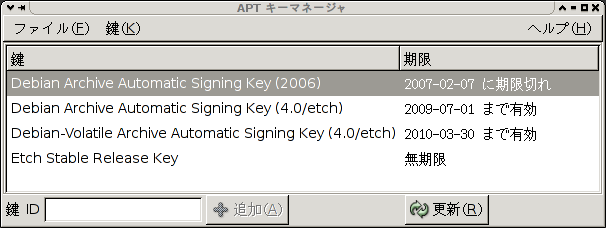
\includegraphics[width=8cm]{image200709/gui-apt-key.png}
 \caption{gui-apt-key}
 \end{center}
 \end{figure}
 \end{itemize}
\end{frame}

\begin{frame}[containsverbatim]{apt-spy}
\begin{itemize}%[<+->]
 \item ネットワークの情報から最適な apt-line を生成することができるツール
   \begin{commandline}
# apt-spy -d stable -s JP
   \end{commandline}

 \item 今は cdn.debian.or.jp があるのですでに役目は終えた気がします。
 \end{itemize}
\end{frame}

\begin{frame}[containsverbatim]{auto-apt}
\begin{itemize}%[<+->]
 \item 世間では検索用のツールとして有名
 \begin{commandline}
 % auto-apt upate
 % auto-apt search stdio.h
 usr/include/stlport/stdio.h     libdevel/libstlport5.1-dev
 usr/include/fcgi_stdio.h        libdevel/libfcgi-dev
 usr/include/H5FDstdio.h libdevel/libhdf5-lam-dev,libdevel/libhdf5-mpich-dev,\
  libdevel/libhdf5-serial-dev
 usr/include/stdio.h     libdevel/libc6-dev
 \end{commandline}
 \item しかし、ファイル検索用として apt-file というコマンドがある
 \end{itemize}
 \end{frame}
\begin{frame}[containsverbatim]{auto-apt}
 \begin{itemize}%[<+->]
 \item  本来はコマンド実行時に足りないファイルをパッケージをから探しだし、インストールしてくれるツール
 \begin{commandline}
 # auto-apt run ./configure
 \end{commandline}
 \end{itemize}
\end{frame}

\begin{frame}{cron-apt}
 \begin{itemize}%[<+->]
 \item apt を cronで動作させるためのツール

	わざわざ cron で書かなくてもよい

 \item apticron

	aptitude の cron-apt 版ではなく、セキュリティアップデート情報
	をメールで送信してくれるツール。名前にだまされるな。

 \end{itemize}
\end{frame}

\begin{frame}{apt-proxy / apt-cacher}
 \begin{itemize}%[<+->]
 \item Debian パッケージのキャッシングプロキシを構築するパッケージ
 \begin{figure}[h]
使用しない場合

 \begin{center}
 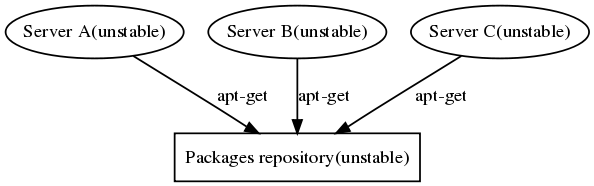
\includegraphics[width=10cm]{image200709/apt-proxy.png}
 \end{center}
 \end{figure}
 \end{itemize}
\end{frame}

\begin{frame}{apt-proxy / apt-cacher}
 \begin{figure}[h]
使用した場合
 \begin{center}
 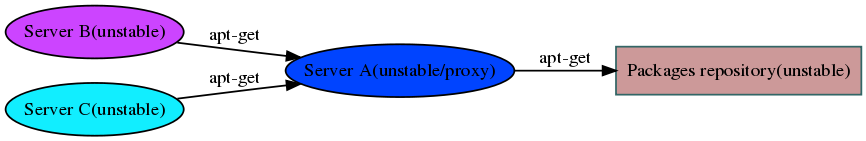
\includegraphics[width=12cm]{image200709/apt-proxy-e.png}
 \end{center}
 \end{figure}
\end{frame}


\begin{frame}[containsverbatim]{apt-ftparchive}
 \begin{itemize}%[<+->]
 \item Packages.gz などのパッケージ情報用ファイルを作成するためのツール

 自分で作ったパッケージを apt-line として公開したい場合などに使用する。
\begin{commandline}
  % apt-ftparchive packages . | gzip -9 > Packages.gz
  % apt-ftparchive sources . | gzip -9 > Sources.gz
  % apt-ftparchive release . > Release
\end{commandline}
\end{itemize}
\end{frame}

\begin{frame}[containsverbatim]{apt-sortpkgs}
 \begin{itemize}%[<+->]
 \item Packages.gz および Sources.gz ファイルをソートする

   apt-ftparchive で作成したファイルはソートされていない場合がある。
   apt-sortokgs を使い、アルファベット順にソートする。

\begin{commandline}
 % apt-sortpkgs Packages > Packages.sort
\end{commandline}
  \end{itemize}
\end{frame}

\begin{frame}[containsverbatim]{apt-extracttemplates}
 \begin{itemize}%[<+->]
 \item Debian パッケージから debconf の設定とテンプレート情報を抽出する

\begin{commandline}
 % wget http://http.us.debian.org/debian/pool/main/x/xorg/ \
xserver-xorg_7.3~rc1_all.deb
 % apt-extracttemplates xserver-xorg_7.3~rc1_all.deb
 % ls
 xserver-xorg.config.34261
 xserver-xorg.template.34260
\end{commandline}
 \end{itemize}
\end{frame}

\begin{frame}[containsverbatim]{apt-build}
 \begin{itemize}
  \item apt-get 感覚でパッケージをビルドできるツール

  \item apt-build を使用せず、Debian パッケージをリビルドする場合
   \begin{commandline}
 % apt-get update
 % apt-get source hello
 % cd hello-x.x
 % debuild -us -uc
 % sudo dpkg-i ../hello_xxxx.deb
   \end{commandline}
 \end{itemize}
\end{frame}

\begin{frame}[containsverbatim]{apt-build}
 \begin{itemize}%[<+->]
  \item apt-build を使用した場合
   \begin{commandline}
 % sudo apt-build build-source hello
   \end{commandline}

 \item apt-build の設定ファイル
  \begin{commandline}
 /etc/apt/apt-build.conf
  \end{commandline}
 \end{itemize}
\end{frame}

\begin{frame}{apt-cross}
 \begin{itemize}%[<+->]
 \item クロスコンパイル用 apt

 Debian package を apt を使い、クロスコンパイル用パッケージに変換してインストールする。

 \end{itemize}
\end{frame}


\begin{frame}{apt-cross}
 \begin{figure}[h]
apt-cross を使用しない場合
 \begin{center}
 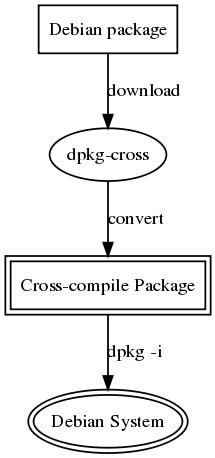
\includegraphics[width=12cm]{image200709/apt-cross.png}
 \end{center}
 \end{figure}
\end{frame}


\begin{frame}{apt-cross}
 \begin{figure}[h]
apt-cross を使用した場合
 \begin{center}
 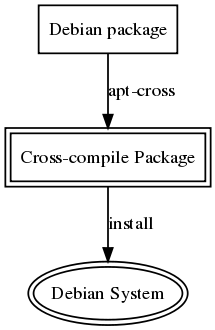
\includegraphics[width=12cm]{image200709/apt-cross-e.png}
 \end{center}
 \end{figure}

\end{frame}


\begin{frame}{apt-transport-https}
 \begin{itemize}%[<+->]
 \item https 経由で apt-get を行うためのツール

 apt-get はftp/http で行うが、このパッケージを使うことによって
 https 経由で apt を行うことができるようになる。
 \end{itemize}
\end{frame}

\begin{frame}{apt-zip}
 \begin{itemize}%[<+->]
 \item リムーバブルメディアの ZIP からの apt をサポートするためのツール
 \begin{figure}[h]
 \begin{center}
 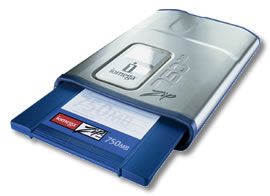
\includegraphics[width=3cm]{image200709/zip_750usb.jpg}
 \end{center}
 \end{figure}

 同じようなツールで apt-cdrom がありますが、違いがいまいちわかりません。
 \end{itemize}
\end{frame}

\begin{frame}[containsverbatim]{aptsh}
 \begin{itemize}%[<+->]
 \item apt の操作をができる Shell.
 \item 使い方
\begin{commandline}
% sudo aptsh
Generating and mapping caches...
Reading commands history...
aptsh>
\end{commandline}

\end{itemize}
\end{frame}

\begin{frame}[containsverbatim]{aptsh}
例えば
\begin{commandline}
% ls
glibc-cross-sh4
snort-rules-default
python-tclink
pipenightdreams
osgcal-doc
mpg123-alsa
...
diatheke
darkice
cyrus-admin-2.2
aspell-bg
libungif4g
libsmpeg0
\end{commandline}
 を実行すると、インストール可能なパッケージ一覧が表示されます。
\end{frame}

\begin{frame}{まとめ}

今回はさわりだけを説明しました。今回の紹介で気になるapt-xxx がありましたら
詳細を説明していきたいと思っています。

\end{frame}

\section{Exim 再発見}
\emtext{Exim 再発見}

\section{事前課題紹介}
\emtext{事前課題の紹介}
% pre work home work

\begin{frame}{事前課題問題}
「あなたがDebianで使っている MTA のこだわりの設定」もしくは「Debian
で利用しているこんな便利な/楽しいメッセージツールあるいは日頃使っていて
気にかかるメッセージ関連ソフトのこの部分」
というタイトルで200-800文字程度の文章を書いてください。というものでした。
その課題に対して下記の内容を提出いただきました。
\end{frame}

\begin{frame}{やまねひでき}
\begin{itemize}
\item その昔、postfix + fml で運用をしていたところ、unstable の postfix
パッケージを入れたら postfix にバグがあって無効な directive を書いたら踏み台
にされたことがありました orz (普通なら無視されるだけなのに、なぜかリレーを受け付
けてしまうのでした。リレーチェックの CGI のページなどで確認はしたのですが…いまだ
に受け付けた理由は不明)

\item そういや fml って fml8 は本当に出てくるのでしょうか。いまだと mailman
が標準メーリングリストドライバなのかな。

\item qmail は捨てたいのですが、いまだに使いたい人とかいるんですよね。ある blog
でソースから入れていていちいちパッケージ入れなきゃいけない、なんてことが書いてあった
ので apt-get build-dep qmail-src で必要そうなパッケージ入れれば良いのに、
と書いたら逆切れされたのもいい記憶です ;-)
\end{itemize}
\end{frame}

\begin{frame}{やまねひでき}
\begin{itemize}
\item ある人は Debian をインストールして最初にするのは nano ではなく vi
をデフォルトエディタにすることと exim を削除して postfix を入れることと言っていましたが、
私も postfix を入れています。理由は単に昔触ったことがあって勘が効くだろうから、というだけ
ですが。

\item 複数 MTA を同時に入れられると良いですよね。

\item spam 対策は非常に大変そうです。spamassassin は入れて手元で運用した事がありますが、
CPU を非常に喰うので中古ノートPCでは問題です。どういう対応が spam 対策として一番良いので
しょうか?
\end{itemize}
\end{frame}


\begin{frame}{本庄}

\textbf{あなたがDebianで使っている MTA のこだわりの設定}
MTAにはPostfixを利用しています。

MTAで特にこだわった設定は行っていませんが、MDAにprocmailを使用し、
ここから添付メールの自動圧縮などを設定したりしています。

\end{frame}

\begin{frame}{濱野}

\textbf{あなたがDebianで使っている MTA のこだわりの設定}
\\
qmail から脱却できないひとりです、exim に超期待。
qmail はちょこっと弄ってエンベロープ To が使用しているメールアドレスじゃ
なかったらその場で SMTP エラーを返してTCP コネクションを切る、というよ
うなことをやっています。backscatter なメールを撒かなくて良いのと spam
が減っているような気分になります。

\end{frame}

\begin{frame}{濱野}
\textbf{Debian で利用しているこんな便利な/楽しいメッセージツール}

最近 ejabberd で遊んでます。ejabberd は Erlang で書かれた jabber サーバー
です。最新の erlang 実行環境 + openssl + ejabberd をソースからコンパイ
ルすると openssl の兼ね合いではまるのですが(古い Erlang だと動く)、
debian package はサクッと動作するのでお手軽です。

\end{frame}

\begin{frame}[containsverbatim]{山本}
\textbf{日頃使っていて気にかかるメッセージ関連ソフトのこの部分}

まず、KSirc について。
KSirc を ISO-2022-JP (JIS) でつかっていると、
以下の (?? 7e) の文字コードのもの 67 個の後に続く文字列が化けます。

蔭 応 改 萱 棄 京 屈 捲 向 込 刷 時 周 償 飾 裾 線 憎 只 寵
逓 到 入 麦 美 服 朋 満 癒 璃 聯 傲 辨 咨 圉 奩 屓 廏 悚 戛
撼 暼 棍 檣 沾 滌 燼 珱 癰 磬 筐 紆 缺 腋 苙 蕈 蝙 襞 譫 蹊
迸 錮 陞 顰 髷 鵈 龠

↓こんなかんじ
\begin{commandline}
<yamamoto> 時?慌修韻襪里?福??
<yamamoto> 周???
\end{commandline}
\end{frame}

\begin{frame}[containsverbatim]{山本}
\textbf{日頃使っていて気にかかるメッセージ関連ソフトのこの部分}

「設定→KSirc を設定→色→強調→kSirc の色コードを削除」
にチェックを入れていると確実に化けるのですが、
チェックを外していても時々化け始めます。

再現条件がいまいち分からず、それに日本語特有なんで、
BTS にも出しずらいのが難点です。

あと、Icedove について。
どうでも良いようなことですが、sid の Icedove のボタンのアイコンが
Thunderbird オリジナルのものと同じなのは気になります(わら
それに、OpenPGP のサインの詳細を知るためのペンアイコンが出ないのも
少々難儀しています
\end{frame}

\begin{frame}{前田}
\textbf{あなたがDebianで使っている MTA のこだわりの設定}

自宅環境では、一つ一つは特に変わった設定はしていませんが、
メールを内部のメールサーバ(B)に集約し、どのクライアントを
使ってもメールを見られるようにしています。

記号の説明と使用しているソフト
\begin{description}
\item[A] 外向けMTA(Postfix)
\item[B] 内部メールサーバ
	(MTA \& MDU \& MUA)(Postfix \& Courier-IMAP \& Fetchmail)
\item[C] 他用途のサーバ (ssmtp)
\item[D] クライアント用PC(Postfix)
\end{description}

\end{frame}


\begin{frame}{前田}
メール送信時
\begin{itemize}
\item C or D → B → A → Internet
 メール受信時(外からの自ドメイン)
\item C → B ← A ← Internet
 メール受信時(自宅内での自ドメイン)
\item C → B ← [A|B|C|D]
 メール受信時(ISPのメール)
\item C → B → ISPメールサーバ
\end{itemize}

C, DはBを、BはAをリレー先にし、A, Bでは自ドメイン当てのみBに向けるようにしています。
ISPからのメールをB(内部メールサーバ)で直接fetchmailで取りに行っているので、
SpamAssassinをBでspamdで動かしています。
Cのメールサーバ以外のサーバでは、Postfixでは機能が多すぎるのでssmtpを使っています。
Dのクライアントでssmtpを使わなかったのは、ネットワークから切り離していると、メールが
ローカルキューに貯まらず、消失してしまうためです。
\end{frame}

\begin{frame}[containsverbatim]{小室}
\textbf{あなたがDebianで使っている MTA のこだわりの設定}

Exim 4 と一緒に ClamAV, SpamAssassin, Mailman を動かしています。
ClamAV/SpamAssassinは
\begin{commandline}
/etc/exim4/conf.d/main/02_exim4-config_options
\end{commandline}
に
\begin{commandline}
av_scanner = clamd:/var/run/clamav/clamd.ctl
spamd_address = 127.0.0.1 783
\end{commandline}
と追加。exim4-daemon-heavyに感謝。
\end{frame}
\begin{frame}[containsverbatim]{小室}
\textbf{あなたがDebianで使っている MTA のこだわりの設定}


後はMailmanのaliasをEximが自動生成してくれるから便利だなとか。
\begin{commandline}
  mailman_router:
    driver = accept
    require_files = MAILMAN_HOME/lists/$local_part/config.pck
    local_part_suffix_optional
    local_part_suffix = -bounces : -bounces+* : \
                        -confirm+* : -join : -leave : \
                        -owner : -request : -admin
    transport = mailman_transport
\end{commandline}
\end{frame}

\begin{frame}{岩松}
\textbf{あなたがDebianで使っている MTA のこだわりの設定}

家で動いているサーバーの MTA は Postfix を使っています。
ライセンスや設定方法などを考えると自動的に Postfix になってしまいました。
特にこだわりの設定は行っていません。
\end{frame}

\begin{frame}{岩松}
\textbf{Debian で利用しているこんな便利な/楽しいメッセージツールあるいは日頃使っていて
気にかかるメッセージ関連ソフトのこの部分}

普段使っているのは ekiga です。一時は家に sip サーバーを立ち上げて遊んでいました。
最近は USB カメラにはまっているので、画像転送用に使っていたりします。
\end{frame}

% (query-replace "\\subsection" "\\end{frame}\\begin{frame}")
% (query-replace "\\subsubsection" "\\textbf")

\section{サマリー}

\begin{frame}{サマリー}

\end{frame}

\section{最近のイベント}
\begin{frame}{最近のイベント}
\begin{itemize}
 \item 10月5-6日 OSC Tokyo/Fall 兼 Debian勉強会
\end{itemize}
\end{frame}

\end{document}
